\documentclass{beamer}

\usepackage{epsfig}
\usepackage{multicol}
\usepackage{geometry}
%\usepackage[dvipsnames]{xcolor}
\usepackage{textcomp}
\usepackage{graphicx}
\usepackage{caption}
\usepackage{subcaption}
\usepackage{amsmath}
\usepackage{tcolorbox}
\usetheme{Boadilla}
\usepackage{pict2e}
\usepackage{tikz}
\usepackage{xcolor}


\title[Traitement du signal numérique]{Traitement du signal numérique - HEI4 IMS}
\author[Antony Bazir]{}

\setlength{\unitlength}{1cm}

\begin{document}


\section{Signaux Numériques}
\begin{frame}
\frametitle{Signaux Numériques}
Les transformées de Laplace et Fourier s'appliquent aux signaux continus. Or, on souhaite traiter des \textbf{signaux numériques...}\\

\vspace{1cm}

\only<2->{
\textbf{Comment définit-on des signaux numériques ?}\\
}

\vspace{1cm}

\only<3->{
\textbf{Signal numérique =  codage + échantillonnage}
}

\end{frame} 

\subsubsection{Codage}
\begin{frame}
\frametitle{Codage}
\textbf{Que vous évoque la notion de codage ?}\\
\vspace{1cm}
\only<2->{
\begin{block}{}
Codage : Mode de répresentation discret de l'amplitude caractérisé par des \textbf{quantas} et une \textbf{dynamique}
\end{block}
}

\end{frame}

\begin{frame}
\frametitle{Codage}
Exemple : Deux manières de coder une fonction rampe de pente 1\\
\vspace{0.3cm}
\only<2->{
\begin{center}
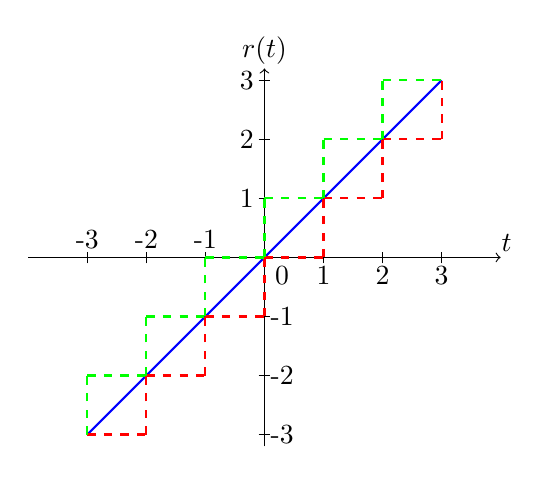
\begin{tikzpicture}
\begin{scope}[scale = 0.75]
\draw[->] (-4,0)-- (4,0);
\draw (0.3,-0.3) node {0};
\draw[->] (0,-3.2)-- (0,3.2);
\draw (4.1,0.25) node {$t$};
\draw (0,3.5) node {$r(t)$};

\draw (1,-0.1)-- (1,0.1);
\draw (1.0,-0.3) node {1};
\draw (2,-0.1)-- (2,0.1);
\draw (2.0,-0.3) node {2};
\draw (3,-0.1)-- (3,0.1);
\draw (3.0,-0.3) node {3};

\draw (-1,-0.1)-- (-1,0.1);
\draw (-1.0,0.3) node {-1};
\draw (-2,-0.1)-- (-2,0.1);
\draw (-2.0,0.3) node {-2};
\draw (-3,-0.1)-- (-3,0.1);
\draw (-3.0,0.3) node {-3};

\draw (-0.1,1)-- (0.1,1);
\draw (-0.3,1) node {1};
\draw (-0.1,2)-- (0.1,2);
\draw (-0.3,2) node {2};
\draw (-0.1,3)-- (0.1,3);
\draw (-0.3,3) node {3};

\draw (-0.1,-1)-- (0.1,-1);
\draw (0.3,-1) node {-1};
\draw (-0.1,-2)-- (0.1,-2);
\draw (0.3,-2) node {-2};
\draw (-0.1,-3)-- (0.1,-3);
\draw (0.3,-3) node {-3};

%r(t)
\draw[thick,blue] (-3,-3)-- (3,3);

\draw[thick,dashed,red] (-3,-3)-- (-2,-3);
\draw[thick,dashed,red] (-2,-3)-- (-2,-2);
\draw[thick,dashed,red] (-2,-2)-- (-1,-2);
\draw[thick,dashed,red] (-1,-2)-- (-1,-1);
\draw[thick,dashed,red] (-1,-1)-- (-0,-1);
\draw[thick,dashed,red] (-0,-1)-- (-0,-0);
\draw[thick,dashed,red] (-0,-0)-- (1,-0);
\draw[thick,dashed,red] (1,0)-- (1,1);
\draw[thick,dashed,red] (1,1)-- (2,1);
\draw[thick,dashed,red] (2,1)-- (2,2);
\draw[thick,dashed,red] (2,2)-- (3,2);
\draw[thick,dashed,red] (3,2)-- (3,3);

\draw[thick,dashed,green] (-3,-2)-- (-2,-2);
\draw[thick,dashed,green] (-3,-3)-- (-3,-2);
\draw[thick,dashed,green] (-2,-1)-- (-1,-1);
\draw[thick,dashed,green] (-2,-2)-- (-2,-1);
\draw[thick,dashed,green] (-1,-0)-- (-0,-0);
\draw[thick,dashed,green] (-1,-1)-- (-1,0);
\draw[thick,dashed,green] (-0,1)-- (1,1);
\draw[thick,dashed,green] (0,0)-- (0,1);
\draw[thick,dashed,green] (1,2)-- (2,2);
\draw[thick,dashed,green] (1,1)-- (1,2);
\draw[thick,dashed,green] (2,3)-- (3,3);
\draw[thick,dashed,green] (2,2)-- (2,3);
\end{scope}
\end{tikzpicture}
\end{center}
}
\vspace{0.3cm}
\only<3->{
Ici le quanta vaut 1 unité et la gamme dynamique est de 6 quanta
}

\end{frame}

\begin{frame}
\frametitle{Codage} 
\textbf{Exercice: Supposons qu'on code un signal d'une amplitude de crête de 5 volts sur 4 bits}\\
\vspace{1cm}
\begin{itemize}
\item<2-> De combien de valeurs dispose-t-on pour coder la gamme dynamique ?  \only<4->{\textbf{16 valeurs: [0,15]}}
\item<3-> Quelle est la valeur d'un quanta/échelon de quantification ? \only<5->{$q$ = \textbf{0.625 V}} 
\end{itemize}

\end{frame} 

\subsubsection{Echantillonnage} 
\begin{frame} 
\frametitle{\'Echantillonnage} 

\textbf{Question : En quoi consiste pour vous l'opération d'échantillonnage ?}

\only<2->{
\begin{block}{}
"L’échantillonnage consiste à représenter un signal fonction du temps $s(t)$ par ses
valeurs $s(nT_e)$ à des instants multiples entiers d’une durée $T_e$, appelée période d’échantillonnage."\footnotesize {M. Bellanger}
\end{block}
}
\end{frame}

\begin{frame}
\frametitle{\'Echantillonnage : Peigne de Dirac}

L'opération d'échantillonnage s'appuie sur la distribution appelée "peigne de Dirac"\\

\vspace{0.7cm} 

 \[ u_{T_e}(t) = \sum_{n = -\infty}^{\infty} \delta(t-nT_e) \]\\
 
\vspace{0.7cm}
On a alors\\

\vspace{0.3cm}
\begin{block}{}
 \[s(nT_e) = s(t) \cdot u_{T_e}(t) \]
\end{block}

\end{frame} 

\begin{frame}
\frametitle{\'Echantillonnage: exemple}
On souhaite échantillonner le signal : $$ g(t) = 0.55\cos(2 t) + 0.45 \cos(4 t + \frac{\pi}{3}) $$ 
\only<2->{
\begin{center}
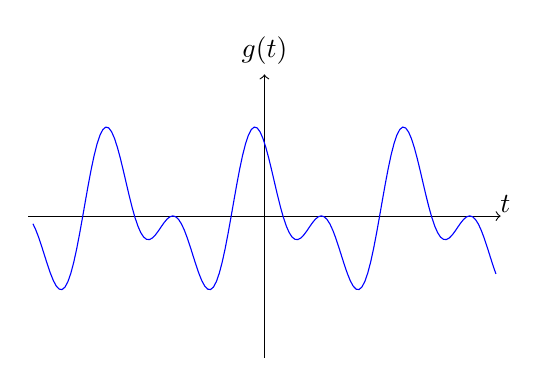
\begin{tikzpicture}
\begin{scope}[scale=0.6]
	\draw[->] (-5,0)-- (5,0);
%\draw (-0.3,-0.3) node {0};
\draw[->] (0,-3)-- (0,3);
\draw (5.1,0.25) node {$t$};
\draw (0,3.5) node {$g(t)$};
%\draw (4.5,-0.3) node {1};

\draw[domain=-4.9:4.9,color=blue,samples=160] plot (\x,{2*(0.55*cos(2*\x r)+ 0.45*cos(2*2*(\x+3.14/12) r))});
\end{scope}
	\end{tikzpicture}
\end{center}
}

\only<3->
{
\begin{block}{}
Quelles sont les composantes en fréquences de ce signal ?
\end{block}
}
\end{frame}

\begin{frame}
\frametitle{\'Echantillonnage: exemple}
On souhaite échantillonner le signal : $$ g(t) = 0.55\cos(2 t) + 0.45 \cos(4 t + \frac{\pi}{3}) $$ 
\only<2->{
\begin{center}
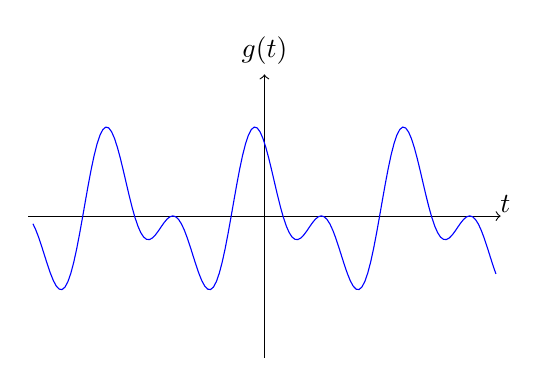
\begin{tikzpicture}
\begin{scope}[scale=0.6]
	\draw[->] (-5,0)-- (5,0);
%\draw (-0.3,-0.3) node {0};
\draw[->] (0,-3)-- (0,3);
\draw (5.1,0.25) node {$t$};
\draw (0,3.5) node {$g(t)$};
%\draw (4.5,-0.3) node {1};

\draw[domain=-4.9:4.9,color=blue,samples=160] plot (\x,{2*(0.55*cos(2*\x r)+ 0.45*cos(2*2*(\x+3.14/12) r))});
\end{scope}
	\end{tikzpicture}
\end{center}
}

\only<3->
{
\begin{block}{}
Quelles sont les composantes en fréquences de ce signal ?
\end{block}
}
\end{frame}

\begin{frame}
\frametitle{\'Echantillonnage: exemple}
On souhaite échantillonner le signal : $$g(t) = 0.55\cos(2 t) + 0.45 \cos(4 t + \frac{\pi}{3}) $$
\begin{columns}[T]
\column{60 mm}
\begin{center}
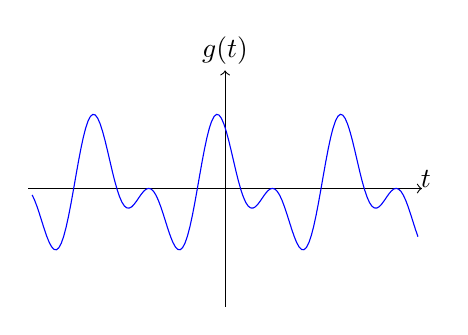
\begin{tikzpicture}
\begin{scope}[scale=0.5,yshift=-1cm]
	\draw[->] (-5,0)-- (5,0);
%\draw (-0.3,-0.3) node {0};
\draw[->] (0,-3)-- (0,3);
\draw (5.1,0.25) node {$t$};
\draw (0,3.5) node {$g(t)$};
%\draw (4.5,-0.3) node {1};

\draw[domain=-4.9:4.9,color=blue,samples=160] plot (\x,{2*(0.55*cos(2*\x r)+ 0.45*cos(2*2*(\x+3.14/12) r))});
\end{scope}
	\end{tikzpicture}
\end{center}

\column{60 mm}

Quelles sont les composantes en fréquence de ce signal ?
\begin{itemize}
\item Méthode "directe" 
\item<2-> Transformée de Fourier 
\end{itemize}
\vspace{0.3cm}
\only<3->
{
$f_1 = \frac{\displaystyle 1}{\displaystyle \pi}$,   $f_2 = \frac{\displaystyle 2}{\displaystyle \pi}$\\
}

\end{columns}
\end{frame}


\begin{frame}
\frametitle{\'Echantillonnage: exemple}
On souhaite échantillonner le signal : $$g(t) = 0.55\cos(2 t) + 0.45 \cos(4 t + \frac{\pi}{3}) $$
\begin{columns}[T]
\column{60 mm}
\begin{center}
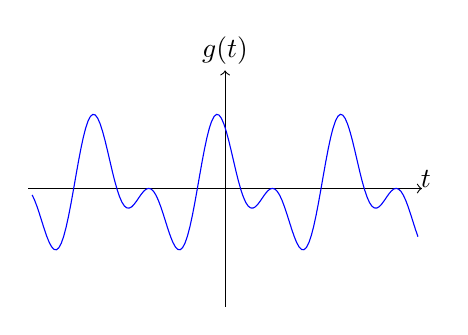
\begin{tikzpicture}
\begin{scope}[scale=0.5,yshift=-1cm]
	\draw[->] (-5,0)-- (5,0);
%\draw (-0.3,-0.3) node {0};
\draw[->] (0,-3)-- (0,3);
\draw (5.1,0.25) node {$t$};
\draw (0,3.5) node {$g(t)$};
%\draw (4.5,-0.3) node {1};

\draw[domain=-4.9:4.9,color=blue,samples=160] plot (\x,{2*(0.55*cos(2*\x r)+ 0.45*cos(2*2*(\x+3.14/12) r))});
\end{scope}
	\end{tikzpicture}
\end{center}

\column{60 mm}

$f_1 = \frac{\displaystyle 1}{\displaystyle \pi}$,   $f_2 = \frac{\displaystyle 2}{\displaystyle \pi}$\\

\vspace{0.3cm}

\only<2->{
Que faut-il avoir à l'esprit lors du choix de $f_e$ (fréquence d'échantillonnage) ?
}

\end{columns}
\end{frame}

\begin{frame} 
\frametitle{\'Echantillonnage: exemple}
\begin{block}{Critère de Shannon}
Pour échantillonner un signal sans perte d'information, il faut que la fréquence d'échantillonnage soit deux fois supérieure à la fréquence maximale présente dans le signal
\end{block}
\only<2->{
\vspace{0.3cm}
$g(t) = 0.55\cos(2 t) + 0.45 \cos(4 t + \frac{\pi}{3}) \rightarrow f_e = $ ?
}

\only<3->{
\vspace{0.3cm}
$g(t) = 0.55\cos(2 t) + 0.45 \cos(4 t + \frac{\pi}{3}) \rightarrow f_e \geq 4/\pi $ 
}

\end{frame}

\begin{frame}
\frametitle{\'Echantillonnage: exemple}
\begin{columns}
\column{60mm}
\begin{center}
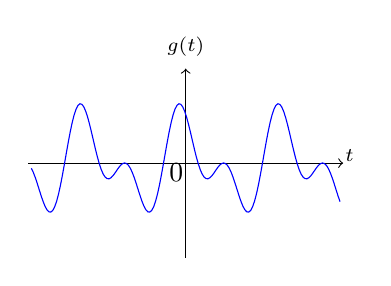
\begin{tikzpicture}
\begin{scope}[scale=0.4]
	\draw[->] (-5,0)-- (5,0);
\draw (-0.3,-0.3) node {0};
\draw[->] (0,-3)-- (0,3);
\draw (5.2,0.25) node {\scriptsize $t$};
\draw (0,3.7) node {\scriptsize $g(t)$};
%\draw (4.5,-0.3) node {1};

\draw[domain=-4.9:4.9,color=blue,samples=160] plot (\x,{2*(0.55*cos(2*\x r)+ 0.45*cos(2*2*(\x+3.14/12) r))});
\end{scope}
	\end{tikzpicture}
\end{center}
\column{60mm}
\begin{center}
\begin{tikzpicture}
\begin{scope}[scale=0.4]
	\draw[->] (-5,0)-- (5,0);
%\draw (-0.3,-0.3) node {0};
\draw[->] (0,-3)-- (0,3);
\draw (5.3,0.25) node {\scriptsize $t$};
\draw (0,3.7) node {\scriptsize $u_{T_e}(t)$};
%\draw (4.5,-0.3) node {1};

\draw[thick,blue] (-4,-0)-- (-4,1);
\draw[thick,blue] (-3.5,-0)-- (-3.5,1);
\draw[thick,blue] (-3,-0)-- (-3,1);
\draw[thick,blue] (-2.5,-0)-- (-2.5,1);
\draw[thick,blue] (-2,-0)-- (-2,1);
\draw[thick,blue] (-1.5,-0)-- (-1.5,1);
\draw[thick,blue] (-1,-0)-- (-1,1);
\draw[thick,blue] (-0.5,-0)-- (-0.5,1);
\draw[thick,blue] (0,-0)-- (0,1);
\draw[thick,blue] (0.5,-0)-- (0.5,1);
\draw[thick,blue] (1,-0)-- (1,1);
\draw[thick,blue] (1.5,-0)-- (1.5,1);
\draw[thick,blue] (2,-0)-- (2,1);
\draw[thick,blue] (2.5,-0)-- (2.5,1);
\draw[thick,blue] (3,-0)-- (3,1);
\draw[thick,blue] (3.5,-0)-- (3.5,1);
\draw[thick,blue] (4,-0)-- (4,1);
\end{scope}
	\end{tikzpicture}
\end{center}

\end{columns}

\begin{center}
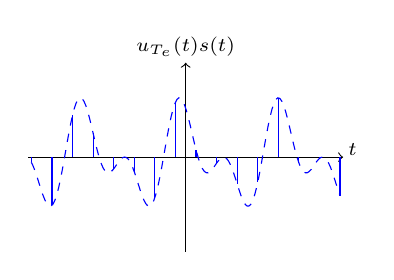
\begin{tikzpicture}
\begin{scope}[scale=0.4]
	\draw[->] (-5,0)-- (5,0);
%\draw (-0.3,-0.3) node {0};
\draw[->] (0,-3)-- (0,3);
\draw (5.3,0.25) node {\scriptsize $t$};
\draw (0,3.5) node {\scriptsize $u_{T_{e}}(t)s(t)$};
%\draw (4.5,-0.3) node {1};

\draw[dashed,domain=-4.9:4.9,color=blue,samples=160] plot (\x,{2*(0.55*cos(2*\x r)+ 0.45*cos(2*2*(\x+3.14/12) r))});

\draw[domain=-4.9:4.9,color=blue,samples=16] plot[ycomb] (\x,{2*(0.55*cos(2*\x r)+ 0.45*cos(2*2*(\x+3.14/12) r))});
%\draw[ domain=0.1:4.9,color=blue,samples=24] plot[ycomb] (\x,{80*abs(sin(5*3.14*\x r -5*3.14*2.5r )/(5*3.14*\x r-5*3.14*2.5 r))});
%\draw[thick,blue] (-4,-0)-- (-4,-0.9);
%\draw[thick,blue] (-3,-0)-- (-3,1);
%\draw[thick,blue] (-2,-0)-- (-2,0);
%\draw[thick,blue] (-1,-0)-- (-1,-1.25);
%\draw[thick,blue] (0,-0)-- (0,1.3);
%\draw[thick,blue] (1,-0)-- (1,-0.15);
%\draw[thick,blue] (2,-0)-- (2,-1.5);
%\draw[thick,blue] (3,-0)-- (3,1.8);
%\draw[thick,blue] (4,-0)-- (4,-0.35);
\end{scope}
	\end{tikzpicture}
\end{center}
\end{frame}

\begin{frame}
\frametitle{\'Echantillonnage: exemple}
Dans les faits, respecter Shannon strictement est un peu limite...\\

\vspace{0.5cm}
\begin{columns}
\column{60mm}
\begin{center}
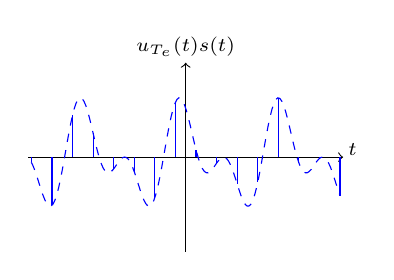
\begin{tikzpicture}
\begin{scope}[scale=0.4]
	\draw[->] (-5,0)-- (5,0);
%\draw (-0.3,-0.3) node {0};
\draw[->] (0,-3)-- (0,3);
\draw (5.3,0.25) node {\scriptsize $t$};
\draw (0,3.5) node {\scriptsize $u_{T_{e}}(t)s(t)$};
%\draw (4.5,-0.3) node {1};

\draw[dashed,domain=-4.9:4.9,color=blue,samples=160] plot (\x,{2*(0.55*cos(2*\x r)+ 0.45*cos(2*2*(\x+3.14/12) r))});

\draw[domain=-4.9:4.9,color=blue,samples=16] plot[ycomb] (\x,{2*(0.55*cos(2*\x r)+ 0.45*cos(2*2*(\x+3.14/12) r))});
%\draw[ domain=0.1:4.9,color=blue,samples=24] plot[ycomb] (\x,{80*abs(sin(5*3.14*\x r -5*3.14*2.5r )/(5*3.14*\x r-5*3.14*2.5 r))});
%\draw[thick,blue] (-4,-0)-- (-4,-0.9);
%\draw[thick,blue] (-3,-0)-- (-3,1);
%\draw[thick,blue] (-2,-0)-- (-2,0);
%\draw[thick,blue] (-1,-0)-- (-1,-1.25);
%\draw[thick,blue] (0,-0)-- (0,1.3);
%\draw[thick,blue] (1,-0)-- (1,-0.15);
%\draw[thick,blue] (2,-0)-- (2,-1.5);
%\draw[thick,blue] (3,-0)-- (3,1.8);
%\draw[thick,blue] (4,-0)-- (4,-0.35);
\end{scope}
\end{tikzpicture}
\end{center}

\column{60mm}
\begin{center}
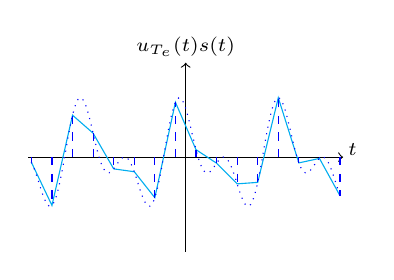
\begin{tikzpicture}
\begin{scope}[scale=0.4]
	\draw[->] (-5,0)-- (5,0);
%\draw (-0.3,-0.3) node {0};
\draw[->] (0,-3)-- (0,3);
\draw (5.3,0.25) node {\scriptsize $t$};
\draw (0,3.5) node {\scriptsize $u_{T_{e}}(t)s(t)$};
%\draw (4.5,-0.3) node {1};

\draw[domain=-4.9:4.9,color=cyan,samples=16] plot (\x,{2*(0.55*cos(2*\x r)+ 0.45*cos(2*2*(\x+3.14/12) r))});

\draw[dotted,domain=-4.9:4.9,color=blue,samples=160] plot (\x,{2*(0.55*cos(2*\x r)+ 0.45*cos(2*2*(\x+3.14/12) r))});

\draw[dashed,domain=-4.9:4.9,color=blue,samples=16] plot[ycomb] (\x,{2*(0.55*cos(2*\x r)+ 0.45*cos(2*2*(\x+3.14/12) r))});
%\draw[ domain=0.1:4.9,color=blue,samples=24] plot[ycomb] (\x,{80*abs(sin(5*3.14*\x r -5*3.14*2.5r )/(5*3.14*\x r-5*3.14*2.5 r))});
%\draw[thick,blue] (-4,-0)-- (-4,-0.9);
%\draw[thick,blue] (-3,-0)-- (-3,1);
%\draw[thick,blue] (-2,-0)-- (-2,0);
%\draw[thick,blue] (-1,-0)-- (-1,-1.25);
%\draw[thick,blue] (0,-0)-- (0,1.3);
%\draw[thick,blue] (1,-0)-- (1,-0.15);
%\draw[thick,blue] (2,-0)-- (2,-1.5);
%\draw[thick,blue] (3,-0)-- (3,1.8);
%\draw[thick,blue] (4,-0)-- (4,-0.35);
\end{scope}
\end{tikzpicture}
\end{center}

\end{columns}

\begin{block}{}
Dans les faits on prend plutôt $f_e > 5 f_{max}$ voire $f_e > 10 f_ {max}$
\end{block}

\end{frame}

\begin{frame}
\frametitle{Impact de l'échantillonnage sur le spectre}

Soit une fonction $g(t)$, $g_{T_e}(nT_e) = \sum_{n = -\infty}^{\infty} g(t)\delta(t-nT_e))$, alors \\

\vspace{1cm} 

\[ TF (\sum_{n = -\infty}^{\infty} g(t)\delta(t-nT_e)) = \frac{1}{T}\sum_{n = -\infty}^{\infty} G(f) \star \delta(f - \frac{n}{T_e}) \] 

\vspace{0.5cm}

\begin{block}{}
Le spectre du signal échantillonnée est constitué de répétitions du spectre du signal original répété tous les $f_e = \frac{1}{T_e}$
\end{block}


\end{frame}

\begin{frame}
\frametitle{Impact de l'échantillonnage sur le spectre}
\vspace{0.5cm}
\begin{columns}
\column{60mm}
\begin{center}
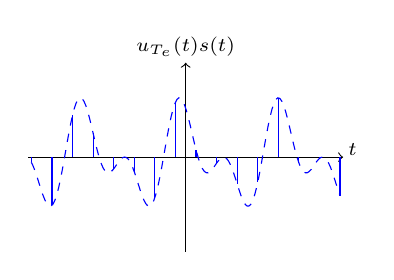
\begin{tikzpicture}
\begin{scope}[scale=0.4]
	\draw[->] (-5,0)-- (5,0);
%\draw (-0.3,-0.3) node {0};
\draw[->] (0,-3)-- (0,3);
\draw (5.3,0.25) node {\scriptsize $t$};
\draw (0,3.5) node {\scriptsize $u_{T_{e}}(t)s(t)$};
%\draw (4.5,-0.3) node {1};

\draw[dashed,domain=-4.9:4.9,color=blue,samples=160] plot (\x,{2*(0.55*cos(2*\x r)+ 0.45*cos(2*2*(\x+3.14/12) r))});

\draw[domain=-4.9:4.9,color=blue,samples=16] plot[ycomb] (\x,{2*(0.55*cos(2*\x r)+ 0.45*cos(2*2*(\x+3.14/12) r))});

\end{scope}
\end{tikzpicture}

\only<2->{
\begin{center}
\begin{tikzpicture}
\begin{scope}[scale=0.4]
	\draw[->] (-5,0)-- (5,0);
\draw (-0,-0.3) node {\scriptsize 0};
\draw[->] (0,0)-- (0,3);
\draw (5.2,0.25) node {\scriptsize $f$};
\draw (0,3.5) node {\scriptsize $|G(f)|$};
%\draw (4.5,-0.3) node {1};


\draw[thick,blue] (1.05,0)-- (1.05,2.5*0.55);
\draw[thick,blue] (2.05,0)-- (2.05,2.5*0.45);
\draw (2.1,-0.8) node {\scriptsize $\frac{2}{\pi}$};
\draw (1.1,-0.8) node {\scriptsize $\frac{1}{\pi}$};

\draw[thick,blue] (-1.05,0)-- (-1.05,2.5*0.55);
\draw[thick,blue] (-2.05,0)-- (-2.05,2.5*0.45);
\draw (-2.1,-0.8) node { \scriptsize $-\frac{2}{\pi}$};
\draw (-1.1,-0.8) node {\scriptsize $-\frac{1}{\pi}$};
\end{scope}
	\end{tikzpicture}
\end{center}

}
\end{center}

\column{60mm}
\begin{center}
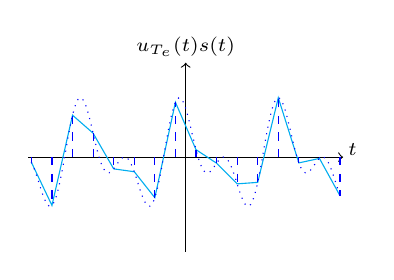
\begin{tikzpicture}
\begin{scope}[scale=0.4]
	\draw[->] (-5,0)-- (5,0);
%\draw (-0.3,-0.3) node {0};
\draw[->] (0,-3)-- (0,3);
\draw (5.3,0.25) node {\scriptsize $t$};
\draw (0,3.5) node {\scriptsize $u_{T_{e}}(t)s(t)$};
%\draw (4.5,-0.3) node {1};

\draw[domain=-4.9:4.9,color=cyan,samples=16] plot (\x,{2*(0.55*cos(2*\x r)+ 0.45*cos(2*2*(\x+3.14/12) r))});

\draw[dotted,domain=-4.9:4.9,color=blue,samples=160] plot (\x,{2*(0.55*cos(2*\x r)+ 0.45*cos(2*2*(\x+3.14/12) r))});

\draw[dashed,domain=-4.9:4.9,color=blue,samples=16] plot[ycomb] (\x,{2*(0.55*cos(2*\x r)+ 0.45*cos(2*2*(\x+3.14/12) r))});

\end{scope}
\end{tikzpicture}

\only<2->{
\begin{center}
\begin{tikzpicture}
\begin{scope}[scale=0.4]
	\draw[->] (-7,0)-- (7,0);
\draw (-0,-0.3) node {\scriptsize 0};
\draw[->] (0,0)-- (0,3);
\draw (7.2,0.25) node {\scriptsize $f$};
\draw (0,3.5) node {\scriptsize $|G(f)|$};
%\draw (4.5,-0.3) node {1};


\draw[thick,blue] (1.05,0)-- (1.05,2.5*0.55);
\draw[thick,blue] (2.05,0)-- (2.05,2.5*0.45);
\draw (2.1,-0.6) node {\scriptsize $\frac{2}{\pi}$};
%\draw (1.1,-0.4) node {$\frac{1}{\pi}$};

\draw[thick,blue] (-1.05,0)-- (-1.05,2.5*0.55);
\draw[thick,blue] (-2.05,0)-- (-2.05,2.5*0.45);
%\draw (-2.1,-0.4) node {$-\frac{2}{\pi}$};
%\draw (-1.1,-0.4) node {$-\frac{1}{\pi}$};


%replica 1
\draw[thick,cyan] (5.05,0)-- (5.05,2.5*0.55);
\draw[thick,cyan] (6.05,0)-- (6.05,2.5*0.45);
%\draw (5.1,-0.4) node {$\frac{5}{\pi}$};
%\draw (6.1,-0.4) node {$\frac{6}{\pi}$};

\draw[thick,cyan] (3.05,0)-- (3.05,2.5*0.55);
\draw[thick,cyan] (2.08,0)-- (2.08,2.5*0.45);
%\draw (3.1,-0.4) node {$\frac{3}{\pi}$};
%\draw (2.1,-0.4) node {$\frac{1}{\pi}$};
\draw (4.1,-0.8) node { \scriptsize $\frac{4}{\pi}$};


%replica 2
\draw[thick,cyan] (-5.05,0)-- (-5.05,2.5*0.55);
\draw[thick,cyan] (-6.05,0)-- (-6.05,2.5*0.45);
%\draw (-5.1,-0.4) node {$-\frac{5}{\pi}$};
%\draw (-6.1,-0.4) node {$-\frac{6}{\pi}$};

\draw[thick,cyan] (-3.05,0)-- (-3.05,2.5*0.55);
\draw[thick,cyan] (-2.08,0)-- (-2.08,2.5*0.45);
%\draw (-3.1,-0.4) node {$-\frac{3}{\pi}$};
%\draw (2.1,-0.4) node {$\frac{1}{\pi}$};
\draw (-4.1,-0.8) node {\scriptsize $-\frac{4}{\pi}$};
\end{scope}
	\end{tikzpicture}
\end{center}
}
\end{center}

\end{columns}

\only<3->{
\begin{block}{}
On voit que les répliques du spectre se touchent. On est à limite du \textbf{repliement de spectre}
\end{block}
}

\end{frame}

\subsection{Transformée en $z$}
\begin{frame}
\frametitle{Transformée en $z$: Définition}
Transformées de Fourier et de Laplace $\rightarrow$ analyse systèmes à fonctions continues\\

\vspace{0.3 cm}

\only<2->{
Transformées en Z $\rightarrow$ analyse systèmes à fonctions discrètes (numériques)\\
}


\only<3->{
\vspace{0.3 cm}
Soit $s[n]$ un signal discret, \\
\[TZ\{ s \}(z) = \sum_{n = -\infty}^{\infty} s_{T_e}[n] z^{-n} \]
}
 \vspace{0.3 cm}

\only<4->{
Tout comme la transformée de Laplace il existe aussi une variante monolatérale:

\[TZ\{ s \}(z) = \sum_{n = 0}^{\infty} s_{T_e}[n] z^{-n} \]
}

\end{frame} 

\begin{frame}
\frametitle{Transformée en $z$: Définition}
\[TZ\{ s \}(z) = \sum_{n = 0}^{\infty} s_{T_e}[n] z^{-n} \]

\vspace{0.3 cm} 
\only<2->{
fonction de $t$ \textbf{échantillonnée} $\rightarrow$ fonction de $z$ \textbf{continue}\\
}
\vspace{0.3 cm} 
\only<3->{
La transformée en $z$ est une fonction \textbf{complexe}
}

\end{frame} 

\begin{frame}
\frametitle{Propriétés de la transformée en $z$}
Par construction, même propriétés que Laplace et Fourier\\
\vspace{0.4cm}

\begin{itemize}
\item<2-> Linéarité \only<3->{: \[TZ(a x_1[n] + b x_2[n]) = a\cdot TZ (x_1[n]) + b\cdot TZ(x_2[n]) \]}
\vspace{0.3cm}
\item<4-> Convolution \only<5->{: \[TZ(x_1[n] \star x_2[n]) = TZ(x_1) TZ(x_2)\]}
\vspace{0.3cm}
\item<6-> Décalage temporel \only<6->{: \[ TZ\{x[n-k]\} = X(z)\cdot z^{-k} \]}
\end{itemize}

\end{frame}

\begin{frame} 
\frametitle{Quelques transformées en $z$ usuelles}
Soit $\delta [n]$ l'impulsion de Kronecker,
\vspace{0.3 cm}
\[TZ\{ \delta[n] \} = \sum_{n = 0}^{\infty} \delta[n] z^{-n}\]

\vspace{0.3 cm}
\only<2->{
\[\sum_{n = 0}^{\infty} \delta[n] \; z^{-n} = z^0 =  1 \]
}

\vspace{0.3 cm}
\only<3->{

\[ \boxed{TZ\{ \delta[n] \} =  1} \]

}
\vspace{0.4cm}
\only<4->{ Résultat similaire en Laplace et en Fourier}

\end{frame}

\begin{frame} 
\frametitle{Quelques transformées en $z$ usuelles}

Soit $u [n]$ l'échelon échantillonné,

\[TZ\{ u[n] \} = \sum_{n = 0}^{\infty} u[n] \; z^{-n}  \]

\vspace{0.3cm}
\only<2->{
\[\boxed{TZ\{ u[n] \} = \sum_{n = 0}^{\infty} z^{-n}  = \frac{1}{1-z^{-1}}} \]

\vspace{0.3cm}
Vrai si $|z|>1$ (série géométrique)

}
\end{frame} 

\begin{frame} 
\frametitle{Quelques transformées en $z$ usuelles}

Soit $n\cdot u [n]$ la rampe échantillonnée,

\[TZ\{ n\cdot u[n] \} = \sum_{n = 0}^{\infty} n \cdot u[n] \; z^{-n} \]

\vspace{0.3cm}

\only<2->{
\[\boxed{TZ\{ n\cdot u[n] \}  = \frac{z^{-1}}{(1-z^{-1})^2}} \]
}

\end{frame}

\begin{frame} 
\frametitle{Quelques transformées en $z$ usuelles}

Soit $\sin(\omega_0 \cdot n )\cdot u [n]$ le sinus échantillonné,

\vspace{0.3cm}

\only<2->{
\[\boxed{TZ\{ \sin(\omega_0 \cdot n )\cdot u [n] \}  = \frac{z^{-1} \sin(\omega_0)}{1-2z^{-1} \cos(\omega_0) +z^{-2}}} \]
}


\end{frame}

\begin{frame}
\frametitle{Quelques transformées en $z$ usuelles}

\begin{enumerate}
\item $\delta[n] \rightarrow  1$ 
\vspace{0.3cm}
\item $u[n] \rightarrow \frac{\displaystyle 1}{ \displaystyle 1-z^{-1}}$
\vspace{0.3cm}
\item $n \cdot u[n] \rightarrow \frac{\displaystyle z^{-1}}{\displaystyle (1-z^{-1})^2} $
\vspace{0.3cm}
\item $\sin(\omega_0 n) \cdot u(n) \rightarrow  \frac{\displaystyle z^{-1} \sin(\omega_0)}{\displaystyle 1-2z^{-1} \cos(\omega_0) +z^{-2}} $
\end{enumerate} 
\vspace{0.5cm}

Fonctions rencontrées fréquemment en traitement du signal.

\end{frame}

\begin{frame}
\frametitle{Transformée en $z$ Lien avec Fourier et Laplace}

Remarque : La transformée en $z$ ne fait pas intervenir la période d'échantillonnage $T_e$...\\

\vspace{1cm}
\only<2->{
Si on souhaite "retrouver" cette variable, il faut repasser de $z$ à Laplace ou Fourier...\\
}

\vspace{1cm}
\only<3->{
\begin{columns}
\column{60mm}
Laplace : 

\[ \boxed{z = e^{sT_e}} \] 

\column{60mm}
Fourier :
\[\boxed{ z = e^{j\omega T_e} = e^{j 2 \pi \nu T_e}} \]
\end{columns}
}

\end{frame}

\subsection{Transformée de Fourier Discrète}
\subsubsection{Définition}
\begin{frame}
\frametitle{Transformée de Fourier...}
On résume... Soit $x[n]$ un signal discret,\\
\vspace{0.3cm}
\only<2->{
\[TZ\{ x[n] \} \rightarrow TF\{x[n]\} =  \sum_{n = -\infty}^{\infty} x[n] e^{-j 2 \pi n \nu T_e}\] \\

\vspace{0.3cm}
Somme infinie... Et variable fréquentielle continue\\
\vspace{0.3cm}
}
\only<3->{
\begin{block}{}
Comment calculer une transformée de Fourier avec un ordinateur ?
\end{block}
}

\end{frame} 

\begin{frame}
\frametitle{Transformée de Fourier...Discrète}
Sur ordinateur ou support numérique, il faut :\\ 
\vspace{0.2cm}
\begin{enumerate}
\item<2-> Sommer sur un nombre fini de termes
\item<3-> Calculer le spectre pour un nombre fini de valeurs en fréquence 
\end{enumerate}

\vspace{0.3cm}
\only<4->{
donc ,
}
\vspace{0.3cm}
\begin{enumerate}
\item<5-> $TF\{ x \}(\nu) = \sum_{n = 0}^{\infty} x[n] \; e^{-j 2 \pi n \nu T_e} \rightarrow  \sum_{n = 0}^{N-1} x[n] \; e^{-j 2 \pi n \nu T_e}$\vspace{0.5cm}
\item<6->$\sum_{n = 0}^{N-1} x[n] \; e^{-j 2 \pi n \nu T_e} \rightarrow  \sum_{k = 0}^{N-1} x[n] \; e^{-j 2 \pi n m \frac{nu_e}{N} T_e }  $
\vspace{0.5cm}
\item<7-> $\sum_{k = 0}^{N-1} x[n] \; e^{-j 2 \pi n m \frac{nu_e}{N} T_e } = \sum_{k = 0}^{N-1} x[n] \; e^{-j 2 \pi n \frac{m}{N} }$
\end{enumerate} 

\end{frame}

\begin{frame}
\frametitle{Transformée de Fourier Discrète (TFD)}
En résumé,\\
\vspace{0.3cm} 
\[ TFD\{ x[n] \} =  \sum_{k = 0}^{N-1} x[n] \; e^{-j 2 \pi n \frac{m}{N}}  \] \\
\vspace{0.4cm}

\vspace{0.3cm}
\begin{itemize}
\item<2-> C'est cette fonction que MATLAB ou Python calcule
\vspace{0.3cm}
\item<3-> formulée ainsi, la TFD comme la transformée en $z$, ne fait pas intervenir $T_e$  
\end{itemize}

\end{frame}

\subsubsection{Lien avec la TFD}
\begin{frame} 
\frametitle{Lien entre TF et TFD}

Transformée de Fourier: $X(f) = \sum_{n = 0}^{\infty} x[n] \; e^{-j 2 \pi n \nu T_e}$' 
\begin{itemize}
\item<2-> Somme infinie sur signal discret
\item<3-> Spectre en fréquence continu (infinité de points)
\end{itemize}
\vspace{1cm}
Transformée de Fourier Discrète :$X_D(m) = \sum_{k = 0}^{N-1} x[n] \; e^{-j 2 \pi n \frac{m}{N} }$
\begin{itemize}
\item<2-> Somme finie ($N$) sur signal discret 
\item<3-> Spectre en fréquence fini et échantillonné sur $N$ points.
\end{itemize}

\end{frame}

\subsubsection{Zero padding}
\begin{frame}
\frametitle{TFD et zero padding}
peu de points dans le signal = peu de points dans le spectre...\\

\vspace{0.2cm}
\[
\begin{bmatrix} x[1] \\ x[2] \\ \vdots \\ x[N] \end{bmatrix} \; -TFD \rightarrow  
\begin{bmatrix} X[1] \\ X[2] \\ \vdots \\ X[N] \end{bmatrix}
\]

\only<2->{Solution:  Zero padding - on ajoute M zéros derrière le vecteur signal
\[
\begin{bmatrix} x[1] \\ x[2] \\ \vdots \\ x[N] \\ 0 \\ \vdots \\ 0 \end{bmatrix} \; -TFD \rightarrow  
\begin{bmatrix} X[1] \\ X[2] \\ \vdots \\  \vdots \\  \vdots \\ X[N+M] \end{bmatrix}
\]}

\end{frame} 

\begin{frame}
\frametitle{TFD et zero padding}

\[
\begin{bmatrix} x[1] \\ x[2] \\ \vdots \\ x[N] \\ 0 \\ \vdots \\ 0 \end{bmatrix} \; -TFD \rightarrow  
\begin{bmatrix} X[1] \\ X[2] \\ \vdots \\  \vdots \\  \vdots \\ X[N+M] \end{bmatrix}
\]
\vspace{0.5cm}

"Interpole" le spectre de façon à avoir plus de points avec le \textbf{même signal}

\only<2->{
\vspace{0.5cm}
\textbf{Attention:} Le zéro padding ne crée pas d'information
}
\end{frame}

\begin{frame}
\frametitle{TFD et zero padding :Exemple}

\begin{columns}
\column{60mm}
\begin{center}
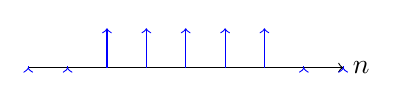
\begin{tikzpicture}
\begin{scope}[scale =0.5]
\draw[->](-4,0)--(4,0) node[right]{$n$};
%\draw(0,-2)--(0,2) node[right]{$x[n]$};

\draw[->,blue](-4,0)--(-4,0);
\draw[->,blue](-3,0)--(-3,0);
\draw[->,blue](-2,0)--(-2,1);
\draw[->,blue](-1,0)--(-1,1);
\draw[->,blue](0,0)--(0,1);
\draw[->,blue](1,0)--(1,1);
\draw[->,blue](2,0)--(2,1);
\draw[->,blue](3,0)--(3,0);
\draw[->,blue](4,0)--(4,0);
\end{scope}
\end{tikzpicture}\\
\vspace{0.4cm}
\only<2->{On rajoute 91 zéros derrière les 9 échantillons pour avoir 100 points dans le spectre}
\end{center}

\column{60mm}
\begin{center}
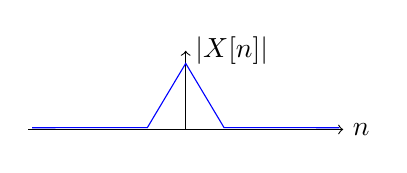
\begin{tikzpicture}
\begin{scope}[scale =0.5]
\draw[->](-4,0)--(4,0) node[right]{$n$};
\draw[->](0,0)--(0,2) node[right]{$|X[n]|$};

\draw[ domain=-3.9:3.9,color=blue,samples=9] plot  (\x,{abs(100*( sin(3.14*\x r  )/(3.14*\x r)))});
\end{scope}
\end{tikzpicture}\\
\vspace{0.9cm}
\only<2->{
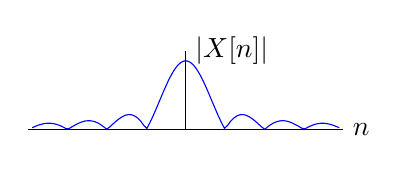
\begin{tikzpicture}
\begin{scope}[scale =0.5]
\draw(-4,0)--(4,0) node[right]{$n$};
\draw(0,0)--(0,2) node[right]{$|X[n]|$};

\draw[ domain=-3.9:3.9,color=blue,samples=100] plot  (\x,{abs(100*( sin(3.14*\x r  )/(3.14*\x r)))});
\end{scope}
\end{tikzpicture}
}
\end{center}
\end{columns}
\vspace{0.5cm}
\only<3->{
En rajoutant des zéros, on se "rapproche" de la transformée de Fourier non-discrète
}
\end{frame}

\begin{frame}
\frametitle{TFD: résumé}
\begin{itemize}
\item TFD calculable par ordi : nombre finis de termes 
\vspace{0.3cm}
\item<2-> Approximation de la TF
\vspace{0.3cm}
\item<3-> Utilisation possible du zéro padding pour rajouter des points au spectre.

\end{itemize}
\vspace{1cm}
Dans tous ces développements on part du principe que l'amplitude est continue mais ce n'est pas exact (codage)
\end{frame}

\subsection{Résumé du chapitre}
\begin{frame}

\frametitle{Résumé du chapitre}
\begin{enumerate}
\item Signaux numériques
\vspace{0.2cm} 
\begin{itemize}
\item<3->  Codage : discrétisation de l'amplitude 
\vspace{0.3cm}
\item<4->  \'Echantillonnage : discrétisation du temps
\vspace{0.3cm}
\begin{itemize} 
\item  Critère de Shannon : $f_e > 2 f_{max}$
\vspace{0.3cm}
\item  Peigne de Dirac et périodisation du spectre $\rightarrow$ \textbf{Repliement spectral}
\end{itemize} 
\end{itemize}
\vspace{0.3cm}
\item<2-> Transformée en $z$ \& Transformée de Fourier discrète
\vspace{0.2cm} 
\begin{itemize}
\item<5->  Définition TZ \& TZ fonctions usuelles 
\vspace{0.3cm} 
\item<6->  Lien avec Fourier : $z = e^{j \pi f T_e}$
\vspace{0.3cm}
\item<7->  Transformée de Fourier discrète et zero-padding
\begin{itemize} 
\item  Limitation du nombre de termes por les supports numériques
\vspace{0.15cm}
\item  Zéro-padding: Ajout de zéros après les échantillons temporels $\rightarrow$ plus de points dans le spectre
\end{itemize} 
\end{itemize}
\end{enumerate}

\end{frame}
\end{document}